\section{Introduction}
\label{sec:introduction}
%\KZ{This para should talk about why you need slogan in e-commerce. You should
%picture a scenario from user point of view, not from system point of
%view.}

%user-needs driven
%The core of e-commerce productions is to establish an 
%effective way of bridging the matching gap
%between user needs and commodities.
To better satisfy shopping needs of users,
e-commerce knowledge graph such as AliCoCo~\cite{luo2020alicoco} has been proposed to  conceptualize implicit user needs explicitly as topic (or concept) nodes like  ``outdoor barbecue'' or ``tools for baking'' and match each shopping need (topic node) to its relevant items.
%a small set of items from an enormous candidate, such that users (even those who do not know exact product) can quickly find the items they need. 
% why we need slogan?
Such user-needs driven knowledge graph makes it more reasonable and convenient to organize billions of items on e-commerce platforms like Alibaba. 
However, equipping downstream applications such as search and recommendation with e-commerce knowledge graph usually require user-oriented textual representation
(called \emph{slogan})  for \emph{topic nodes} demonstration in practical scenarios, 
and we formalize this problem as \emph{slogan generation}.

%concept is short phrase 
%Once an e-commerce concept is activated, its corresponding 
%items are presented to the user which the semantic gap .
%Slogan explore the functions and features of items that matched with user need 
%once a concept is activated in e-commerce scenarios 
%
%
%Equipping downstream applications in e-commerce with such an effective way of organizing items requires 
%
%connecting item features
%recommendation in e-commerce with 
%E-commerce knowledge graph requires 
%to equip 
%across categories
%
%Downstream applications in e-commerce equipped with
%such an effective way of organizing items further improve
%Backed up user-needs driven
%features that promotes user interests
%Equipping with such an effective way of organizing items  benefits various downstream applications in e-commerce. 

%For example, conventional item-based recommendation 
%~\cite{linden2003amazon,sarwar2001item} 
%based on user's historical behaviors is not driven by user needs in the first place, which makes the recommendation results redundant and lack novelty.

A good slogan of a topic node is an informative and more attractive rewrite of the original topic words.
\figref{fig:example} illustrates an example of slogan generation applied in the scenario of topic-based recommendation, 
which is a real application practiced in Alibaba.
Backed by AliCoCo, 
topic-based recommendation~\cite{luo2019conceptualize} 
directly recommends topics to users and display cards with corresponding slogans and pictures on mobile pages. Once clicking, it jumps to another page full of associated items.
%provides superior shopping experience to users and is more effective.
%\figref{fig:example} demonstrates the coarse-grained recommendation scenario based on topics.
In \figref{fig:example}, the topic ``glass light-fixture'' is recommended to two users and two slogans need to be generated for display.
In AliCoCo, this topic node is associated with multiple fine-grained product categories such as ``beside lamp'' and ``ceiling light'' (top).
For a coarse-grained topic, each affiliated product category provides a refined perspective (or potential user interest) of represented user need for the selling point exploration.
For example, the right middle of \figref{fig:example} shows a number of items belonging to \emph{bedside lamp}, which enlightens \emph{bright and warm} as a selling point for customers.
An informative and attractive slogan should not only summarize the topic information but also highlight the selling points which may promote user's interests.
Therefore, for user B who has a preference for \emph{bedside lamp} from her long-term behaviors, 
the generated slogan could be \emph{``Lights in Your World, Bright and Warm''}, 
while the slogan of the same topic changes to \emph{``Ceiling Lights in Modern Style, Shining Minimalist Charm''} for user A, who recently viewed some ``Ceiling Lights''.
With different preference categories of different users, 
the generated slogans are different even for the same topic,
which attracts users to make informed decisions and eventually improve shopping experience.
Besides topic-based recommendation, 
such ``personalized'' slogan generation can also benefit other user-needs driven e-commercial applications where topic nodes are displayed directly to users.

%Slogan, as the terms directly displayed on the page, 
%is crucial to demonstrate the topic nodes to customers. 
%%conceptualizing user needs as concept nodes associated with a small set of items across fine-grained categories, which provides superior shopping experience to users. 
%% crucial 12:45
%Generating quality slogans for the recommended topics helps with exploring latent user interests and providing valuable assistance for users, eventually improves user satisfaction, which also matters in other user-needs driven e-commercial applications. 
%% challenge category relevant 13:00
%One of the biggest challenges is, given a topic, to comprehensively interpret the user need and accordingly reflect the selling points of associated items, which depends on bridging the semantic gap between the potential user interests and functionalities (or features) of related items.
%Since items from different categories have different functionalities, it is essential to refine the user need (i.e. topic node) as potential interests according to categorized items in order to conduct better exploration of selling points.

%reflecting selling points in slogans.
% refine users' intention according to 
%features or functionalities of items
%and represent the concept node from both user needs and 
%functions or features of its associated items.
%understand users intentions,
%explore latent user interests
%help them find what they are looking for, and provide
%valuable assistance during their entire shopping process. Different
%from physical stores where salespeople could have a face-to-face
%conversation with customers, online stores in e-commerce heavily
%rely on textual product descriptions to provide crucial product
%information and, eventually, convince customers to buy the recommended
%products.
%a coarse-grained topic against one particular aspect (called \emph{selling point}) each.

% cpv concept 13:20

% in this paper, we ... explore latent user interests ... 13:40

% contribution 14:00

%driven by user needs in the first place, 
%user needs driven item recommendation, one of the major applications in e-commerce, widely
% 引出
%and 
%explanation
%One of the biggest challenges is to timely 
%explore the selling points 
%help users make shopping decisions, .
%
%improve user satisfaction
% existing challenges or problems
%However, 


%better bridge the semantic gap between what users need in their mind and how the items are organized in e-commerce platforms. 
%E-commerce knowledge graph   set~\cite{luo2019conceptualize,}. 
%user needs and categorize items such that users can quickly find the items they need. 
%Most recently, represent user needs
%A better understanding of user needs helps 
%topics as bridging 
%more effective way of organizing items according to user needs.
%provide more desired items for users. 
%显式建立了一条更有效的用户需求到商品的链路
%%%%%%%%%%%%%%%%
%%%%%%%%%%%%%%%%
%Traditionally, e-commerce platforms use CPV ontology as shown in \figref{fig:cpv} 
%More recently, e-commerce platforms explore user needs and explicitly express them as short phrases.
%Backed up on e-commerce knowledge base, 
%topics are introduced as bridging 
%A typical E-commerce knowledge base shown in  \figref{fig:cpv} usually has three named
%entity types,
%including \emph{Category} (\textbf{CG}),  \emph{Property Key} (\textbf{PK}) and \emph{Property Value} (\textbf{PV}).
%
%\begin{figure}[th!]
%	\centering
%	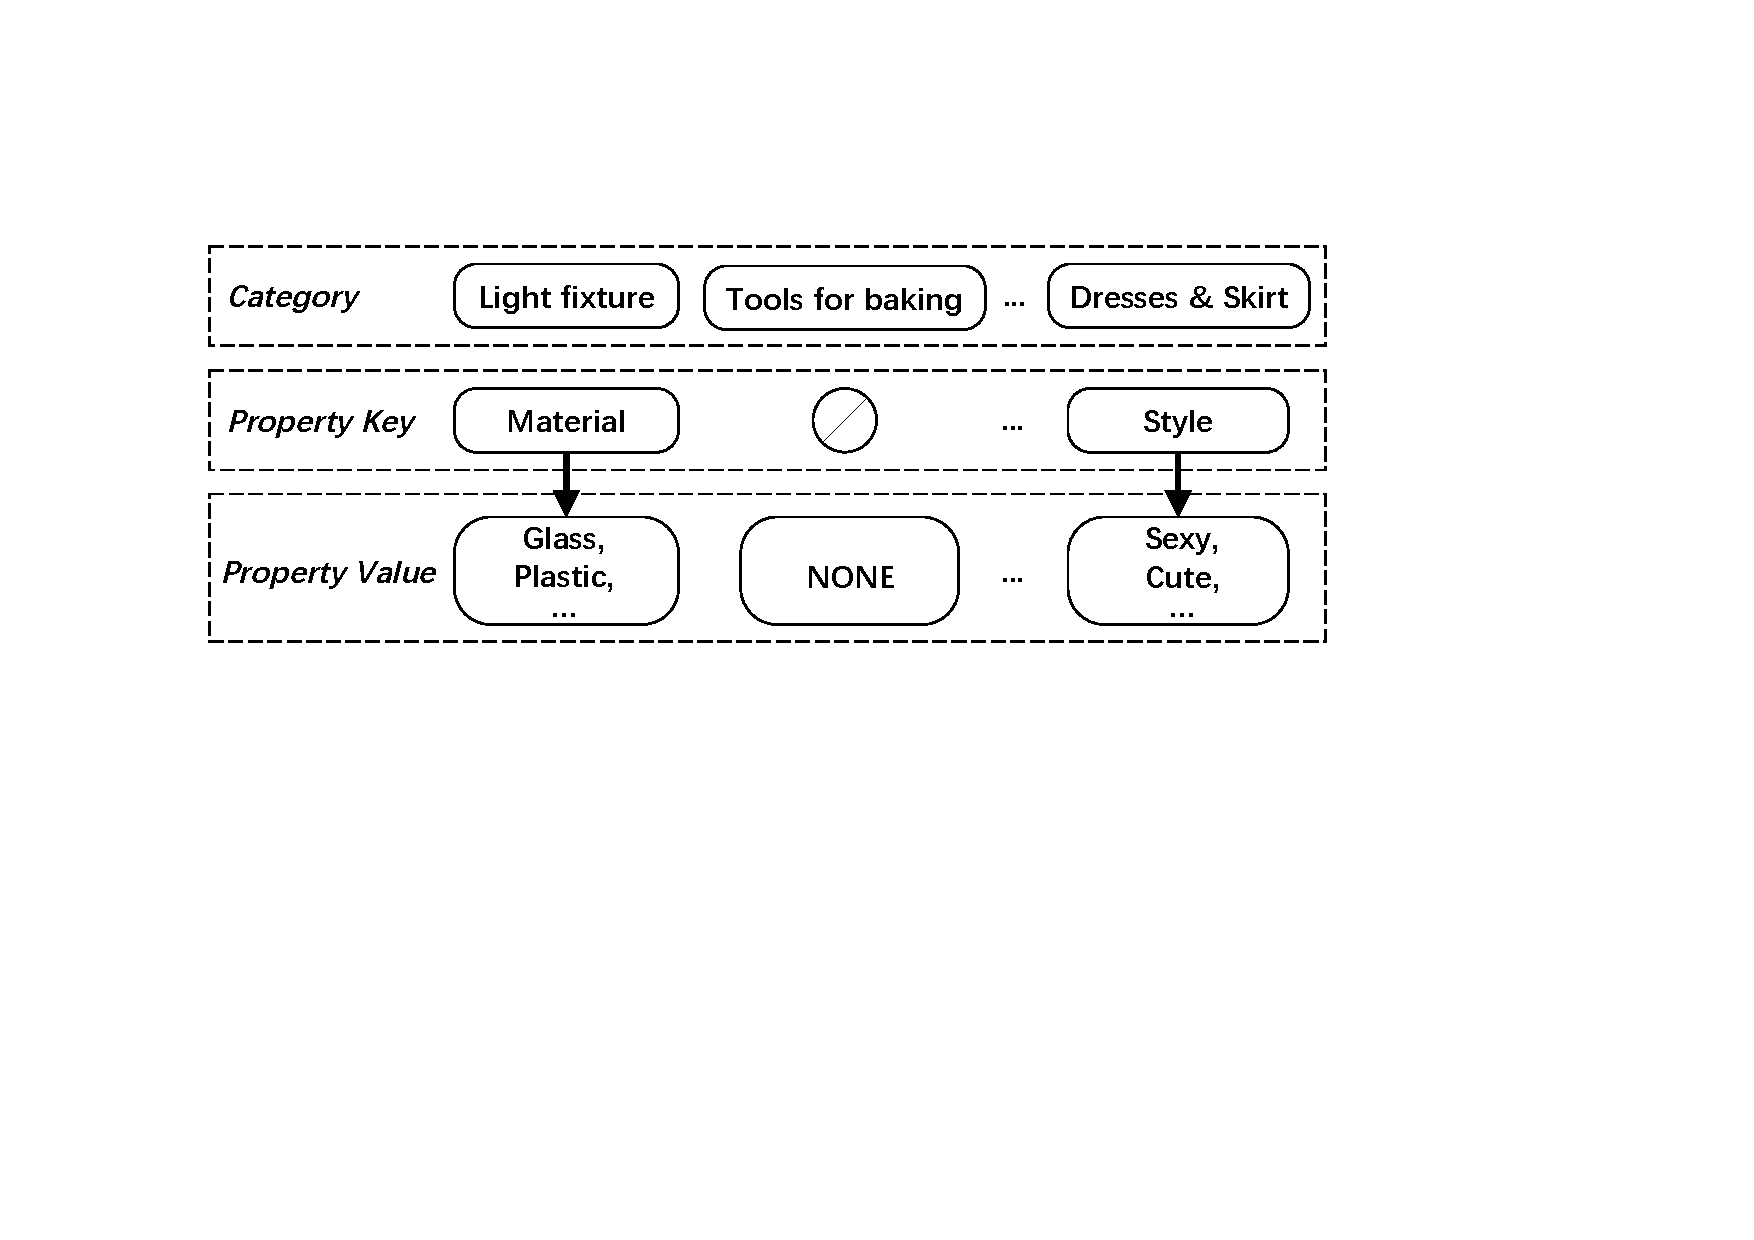
\includegraphics[width=0.95\columnwidth]{figures/cpv2}
%	\caption{The structure of E-commerce knowledge-base.}
%	\label{fig:cpv}
%\end{figure}
%%%%%%%%%%%%%%%%%%
%%%%%%%%%%%%%%%%%%

%It is essential to establish an effective way of organizing
%items according to high-level user needs.
%Traditionally, e-commerce platforms use 
%e-commerce knowledge base including categories 
%and to manage and organize items.
%Nowadays, the exploration and understanding of user needs play fundamental roles in modern e-commercial applications.

%Traditionally, e-commerce platforms use catalogs to organize and manage products which is vital to 
%Nowadays, further exploring and understanding user needs are critical in modern e-commercial applications.
%Most recently, topic-based recommendation is proposed
%to 
%Knowing what users need helps e-commerce product search return more satisfied 


\cut{
%Usually, the topic candidates are built from frequent phrases collected via 
%thoroughly analyzing query logs and product titles in order to cover as many user interests as possible.
%We leverage E-commerce knowledge base to constrain topics
%to a phrase which consists of a \emph{Category} 
%modified by a reasonable Property Value.
We first collect frequent phrases from 
query logs and product titles
in order to cover as many
user interests as possible.
Then, we construct topics from those phrases using E-commerce knowledge base.
%which makes it more reasonable and more convenient to organize items for topics.
The E-commerce knowledge base consists of three named 
entities:
%There are three named entity types in typical E-commerce knowledge base,
%there are three named entity types:
\emph{Category} (CG), \emph{Property Key} (PK) and \emph{Property Value} (PV). 
As shown in \figref{fig:cpv},
``Light fixture" is a Category, 
while ``Material" denotes a Property Key, which is the name of one product property.
``Glass"  and ``Plastic" are concrete property values of ``Material".
We constrain the topic to a phrase which consists of a Category modified by a reasonable Property Value.
Following this constraint, the topic can be associated with 
a set of items belong to the Category with the corresponding Property Value.
For example, ``glass light fixture" is a satisfied topic,
which the Category ``light fixture" is modified
by the concrete Property Value ``glass" of its 
corresponding product property ``Material".
Note that, ``Tools for baking" in \figref{fig:cpv}
also represents a topic which can be seen as the Category
``Tools for baking'' modified by an empty Property Value. 
}



%In the real implementation of recommendation, E-commerce platforms (such as Taobao~\footnote{http://www.taobao.com} App)
%usually combine item-based recommendation with topic-based recommendation.
%Among normal recommended items, the recommended topic is displayed to users as a card with its textual description and 
%the picture of a representative item (\figref{fig:example} left). 
%Taobao App incorporates the topic-based recommendation 
%into recommendation system to satisfy the scenario of coarse-grained recommendation.
%As shown in \figref{fig:topic} \textbf{PLACEHOLDER},
%the topic ``glass light fixture" is displayed to users as a card with
%its textual description and the picture of a representative item (left).
%Once a user clicks on it, he will enter into another page (right) where
%different items satisfied the needs of ``glass light fixture" are displayed.
%Such textual descriptions of topics are like salespeople,
%that is critical to demonstrate the recommended topics to customers.
%Quality textual descriptions attract users' attention, promote users' interests and eventually convince users to buy the recommended products.
%An informative and attractive textual description summarizes topic information and 
%highlights features of associated items which could help 
%users make an informed decision as well as promote users' interests and eventually improve the likelyhood of purchase.
%An informative and attractive textual description summarizes
%topic information and highlights \emph{selling points} of associated
%items which could promote users' interests as well as help users make an informed decision and eventually improve shopping experience.
%A selling point is supposed to highlight common property or function shared by items.
%For example, \emph{Boho style} (property) dresses, shoes and handbags make customer enjoying \emph{cool summer}.
%\figref{fig:example} (right bottom) shows a number of items belong to \emph{bedside lamp} (category or function) enlighting \emph{bright and warm} as a selling point for customers.
%For example, \figref{fig:boximiya} shows a number of items with common property Boho style enlighting \emph{cool summer} as a selling point for customers.
%Thus, the property or category usually need to be provided as a hint to craft quality slogans.

% 
%We suppose that items of  same fine-grained category shared common properties are 
%Items shared common properties are supposed to explore those selling points. Such selling points are explored from items shared common properties or use  Thus, a coarse-grained topic could be decomposed into various focuses referring to different selling points by its associated fine-grained categories.
%Given a topic, multiple slogans could be generated which highlight different features (or selling points) of associated items across 
%fine-grained categories. 
%However, until now, most of the textual descriptions for topics in the online shopping platforms
%namely \emph{slogan},
%are still created manually, 
%which is tedious, time-consuming, and less effective.

%On the other hand, such slogans should be personalized based on the item preferences
%which highlights the selling points to users
%and promotes their interests accordingly.

%We formulate it as a text-to-text generation problem.
%Specially, the system can intelligently generate quality slogans for a specific topic based on the given topic information and item preferences.

\begin{figure*}[th!]
	\centering
	\includegraphics[width=1.8\columnwidth]{figures/cloud}
	\caption{An motivating example of \emph{slogan generation} applied in topic-based recommendation on Alibaba e-commerce platform. For the same topic, we generate different slogans under different category preferences to display for different users.}
\label{fig:example}
\end{figure*}



%We formulate personalized slogan generation as a text-to-text generation task.
%Owing to the tremendous success of
%We suppose that slogans highlights features (or selling points) for the associated items of topics.
%Since items across categories are 
%in order to capture users' intentions and further promote user's interests.
%Each topic conceptualizes user interests and is associated with a bunch of items across 
%fine-grained categories and brands.
%quality slogans for topics are supposed to summarize topics' information and expose features or selling points of associated items.
%One of the biggest challenges is to explore features 
%for the associated items of topics and express 
%those features as specific selling points in generated slogans to further extend the user interests implied by the topic.
Crafting a successful slogan for specific topic is tedious and highly time-consuming.
In this paper, we focus on automating the slogan generation
for online shopping in e-commerce,
which is a relative new problem. 
The most related works are product title generation~\cite{suzuki2011automatic,mathur2017generating,de2018generating}
and product description generation in E-commerce~\cite{langkilde1998generation,wang2017statistical}. Most prior works are based on templates and traditional statistical frameworks which are suffered from incoherence and lack of diversity. None of the previous related works except for Chen et al.~\cite{ChenLZYZ019} extends the powerful encoder-decoder framework, hence are
%Previous related works are mainly use templates or statistical methods which are 
insufficient to generate quality titles or descriptions and achieve satisfying performance.
On the other hand, convolutional sequence-to-sequence (Seq2Seq) learning has been achieved tremendous success in many text generation applications, such as machine translation~\cite{wang2017statistical,chen2018stable,song2018double,wu2019pay},
abstractive document summarization~\cite{fan2017controllable,liu2018controlling,narayan2018don},
language modeling~\cite{baevski2018adaptive},
story generation~\cite{fan2018hierarchical,fan2019strategies}
and dialogue~\cite{miller2017parlai,dinan2018wizard}.
Owing to this success, 
we extend the effective convolutional Seq2Seq framework~\cite{ott2019fairseq}
and propose a 
\textbf{S}emantics-enhanced \textbf{S}logan \textbf{G}eneration (or SSG) 
model to automatically generate quality slogans for 
online shopping needs.
SSG introduces \emph{item preferences} 
to explore selling points of categorized items and promote potential user interests, then proposes a knowledge-enhanced module which
incorporates \emph{is-a} knowledge for better contextualized representations,
and eventally generates more accurate and attractive slogans.

To provide a dataset for the automatic slogan generation,
we construct and make publicly available a new dataset from Taobao\footnote{http://www.taobao.com}.
The dataset contains 3,555 instances in total, including 857 online topics.
We also retrieve the \emph{is-a} knowledge
from AliCoCo and the involved \emph{is-a} knowledge will be released together with the dataset.

The contributions of this paper are summarized below:
\begin{itemize}
	\item We define a new problem called slogan generation, to generate accurate and attractive slogans for shopping needs in e-commerce, which benefits downstream applications such as item recommendation.
	\item We propose a novel model based on sequence-to-sequence learning, 
	which utilizes item preferences and further incorporates the hypernym-hyponym semantic knowledge to improve the quality of generated slogans. Extensive experiments show that our approach outperforms several baselines by a substantial margin.
	\item We create a new dataset for automating slogan generation.
	We intend to release this dataset as well as the implementation of the proposed method for future work in this research area. 
\end{itemize}


%we build various preferred item sets for topics to represent users' preferences accordingly
%by introducing category ontology in E-commerce.
%Such item sets reflect different focuses and potential interests of users.

%讲一下personalize
%users needs - topic - items
%user preferences - secondary category - items


%The most related work are about product description generation and 
%title generation for browse pages.
%
%We introduce the category ontology 
%In topic-based recommendation, a topic bridges user needs and its associated items.
%Similarly, user preferences to a specific topic can be expressed by  
%Similarly, category ontology is introduced as potential focuses
%connecting user preference and items.





%It is necessary to make the slogan focuses adapted to 
%the selling points conducting by users' preferences of items.
%
%A set of associated items represents the users' needs
%by summarizing and con
%A set of preferred items which relevant to a specific topic
%can represent the users' preferences 
%It is reasonable to represent the users' preferences
%of a specific topic as a set of preferred items
%which are relevant to the topic. 
%Besides, such item preferences 
%Different from exploring users' preference from private information,
%we represent the preferences as a set of preferred items relevant to
%a specific topic.
%The system is expzected to explore selling points from 
%the topic and the provided preferred items,

%\begin{figure}[th!]
%	\centering
%	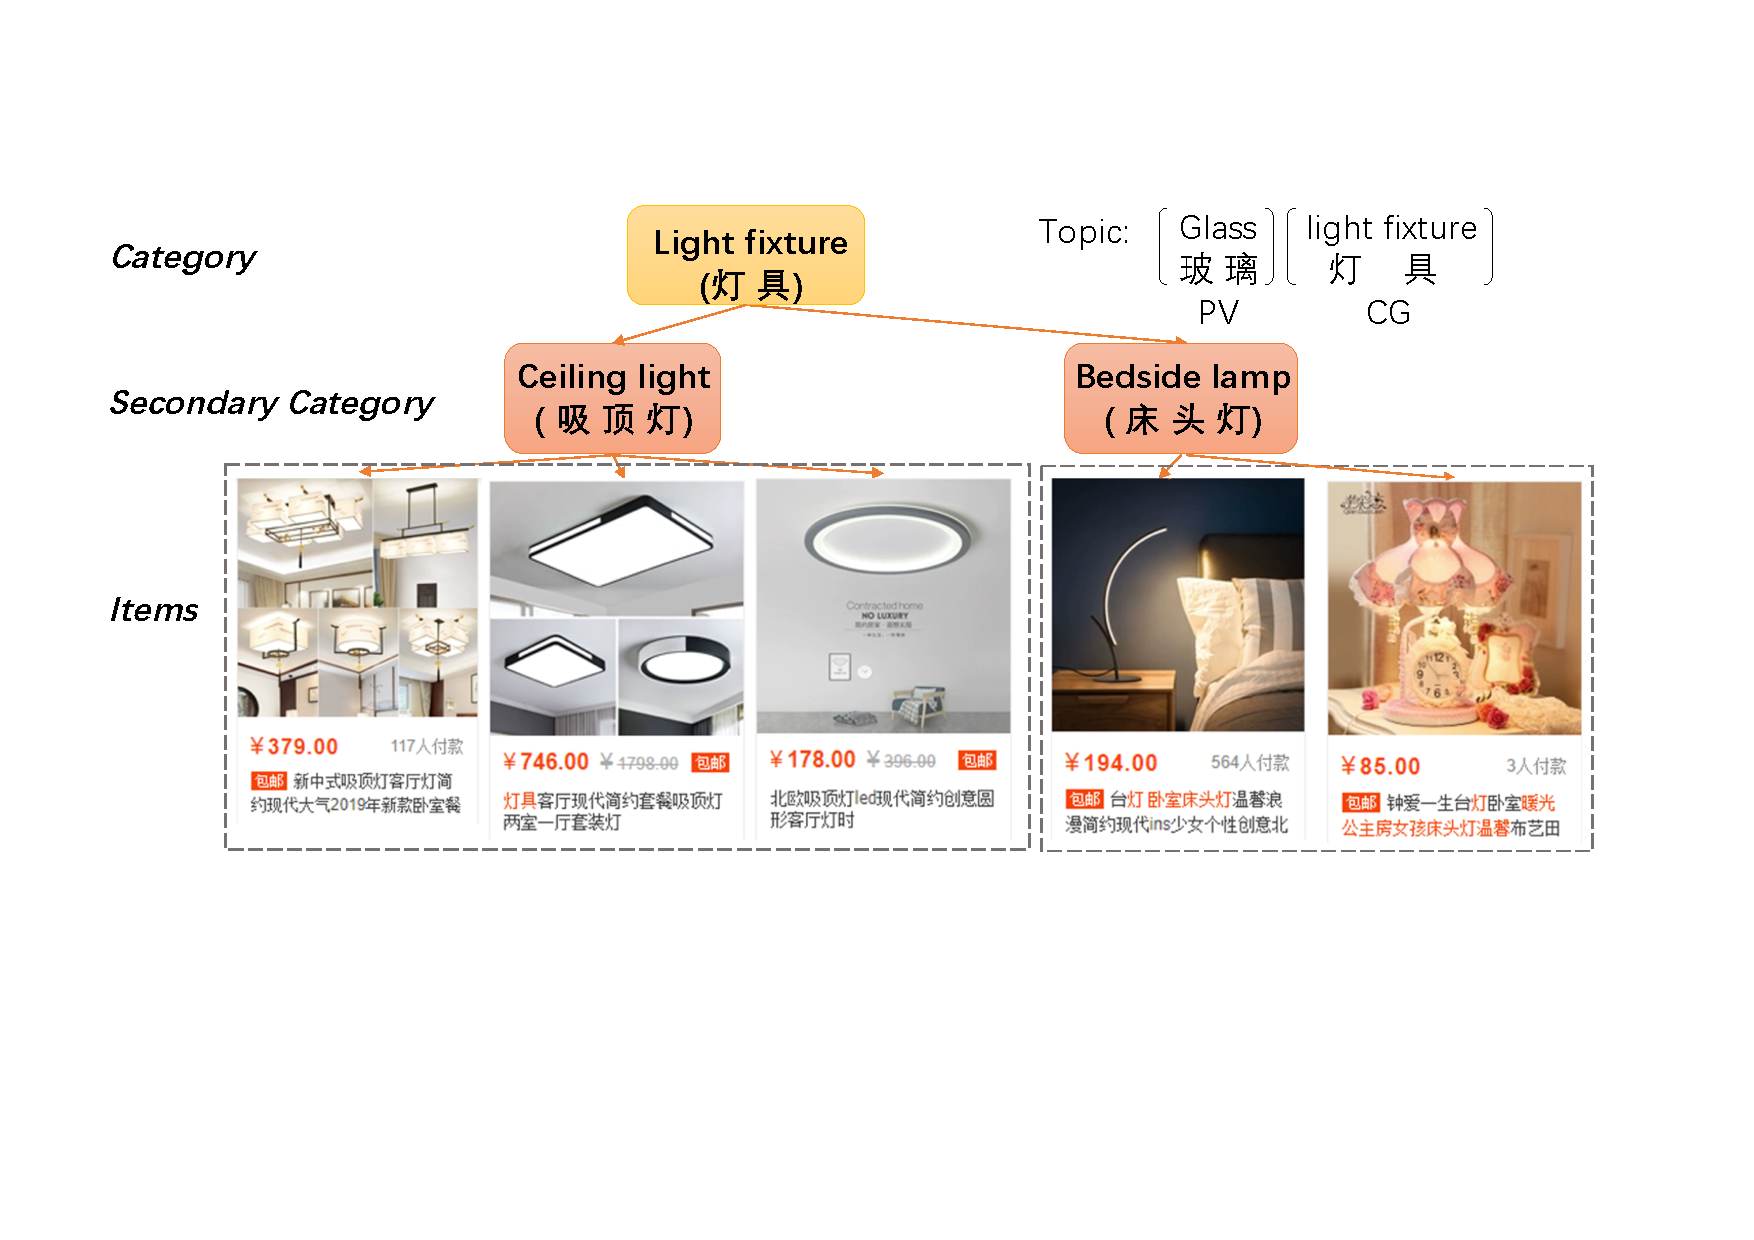
\includegraphics[width=0.95\columnwidth]{figures/cate8}
%	\caption{An example of category structure in E-commerce.}
%	\label{fig:cate}
%\end{figure}




%One of the biggest challenges of recommendation in E-commerce is to 
%efficiently  in an accurate and attractive way.


%说为topic生成标题的重要性

%item-specific details
%attract customer's attention and transfer it to purchase
%别人是怎么做的 局限性在哪


%In this paper, 
%我们要做的是啥
%说明下我们的topic是啥
%我们准备怎么做

%最后总结一下我们的贡献是啥

%related work
%item-based recommendation 展示: product description generation
%topic-based recommendation 展示: slogan generation

%E-commerce platforms traditionally present and recommend items to users using titles and demo pictures from on-line merchants that describe items information.  
% limitations

%To resolve these limitations, instead of \emph{item-based} presentation and recommendation, recent works focus on exploring user needs and propose \emph{topic-based} presentation and recommendation~\cite{}.



%[ebay emnlp 2018] Generating E-Commerce Product Titles and Predicting their Quality
%[kdd 2019] Towards Knowledge-Based Personalized Product Description Generation in E-commerce
%[ICML 2019] Generative Adversarial User Model for Reinforcement Learning Based Recommendation System
